\documentclass[a4paper, man, floatsintext]{apa6}
\usepackage{lmodern}
\usepackage{amssymb,amsmath}
\usepackage{ifxetex,ifluatex}
\usepackage{fixltx2e} % provides \textsubscript
\ifnum 0\ifxetex 1\fi\ifluatex 1\fi=0 % if pdftex
  \usepackage[T1]{fontenc}
  \usepackage[utf8]{inputenc}
\else % if luatex or xelatex
  \ifxetex
    \usepackage{mathspec}
  \else
    \usepackage{fontspec}
  \fi
  \defaultfontfeatures{Ligatures=TeX,Scale=MatchLowercase}
\fi
% use upquote if available, for straight quotes in verbatim environments
\IfFileExists{upquote.sty}{\usepackage{upquote}}{}
% use microtype if available
\IfFileExists{microtype.sty}{%
\usepackage{microtype}
\UseMicrotypeSet[protrusion]{basicmath} % disable protrusion for tt fonts
}{}
\usepackage{hyperref}
\hypersetup{unicode=true,
            pdfauthor={Jana B. Jarecki},
            pdfborder={0 0 0},
            breaklinks=true}
\urlstyle{same}  % don't use monospace font for urls
\usepackage{graphicx,grffile}
\makeatletter
\def\maxwidth{\ifdim\Gin@nat@width>\linewidth\linewidth\else\Gin@nat@width\fi}
\def\maxheight{\ifdim\Gin@nat@height>\textheight\textheight\else\Gin@nat@height\fi}
\makeatother
% Scale images if necessary, so that they will not overflow the page
% margins by default, and it is still possible to overwrite the defaults
% using explicit options in \includegraphics[width, height, ...]{}
\setkeys{Gin}{width=\maxwidth,height=\maxheight,keepaspectratio}
\IfFileExists{parskip.sty}{%
\usepackage{parskip}
}{% else
\setlength{\parindent}{0pt}
\setlength{\parskip}{6pt plus 2pt minus 1pt}
}
\setlength{\emergencystretch}{3em}  % prevent overfull lines
\providecommand{\tightlist}{%
  \setlength{\itemsep}{0pt}\setlength{\parskip}{0pt}}
\setcounter{secnumdepth}{0}
% Redefines (sub)paragraphs to behave more like sections
\ifx\paragraph\undefined\else
\let\oldparagraph\paragraph
\renewcommand{\paragraph}[1]{\oldparagraph{#1}\mbox{}}
\fi
\ifx\subparagraph\undefined\else
\let\oldsubparagraph\subparagraph
\renewcommand{\subparagraph}[1]{\oldsubparagraph{#1}\mbox{}}
\fi

%%% Use protect on footnotes to avoid problems with footnotes in titles
\let\rmarkdownfootnote\footnote%
\def\footnote{\protect\rmarkdownfootnote}

%%% Change title format to be more compact
\usepackage{titling}

% Create subtitle command for use in maketitle
\providecommand{\subtitle}[1]{
  \posttitle{
    \begin{center}\large#1\end{center}
    }
}

\setlength{\droptitle}{-2em}

  \title{}
    \pretitle{\vspace{\droptitle}}
  \posttitle{}
    \author{Jana B. Jarecki}
    \preauthor{\centering\large\emph}
  \postauthor{\par}
      \predate{\centering\large\emph}
  \postdate{\par}
    \date{25 November, 2019}

\usepackage{natbib} \usepackage{threeparttable} \usepackage{booktabs}
\shorttitle{test} \usepackage{setspace}
\AtBeginEnvironment{tabular}{\singlespacing} \usepackage{times}
\usepackage{changes} \definechangesauthor[name={JJ}, color=orange]{jj}
\usepackage{upgreek} \AtBeginDocument{\let\maketitle\relax}

\begin{document}

\textit{Predictions about gamble valuations.}
\added[id=jj]{Figure \ref{fig:fig6}a shows that, as predicted, among the Bayesian participants, those with zero-outcome priors increased their evaluations of p-bets, those with gain priors decreased their evaluations of \$-bets, and RF-type participants remained relatively stable across sample sizes. Statistical analyses by means of a Bayesian generalized linear model\footnote{regressing the (normalized, within-person z-standardized) evaluations on the predictors sample size, gamble type, and learner class (BVU-gain-prior, BVU-loss-prior, RF) with a by-participant random intercept; categorical predictors were effects-coded to facilitate interpretation of interactions.} favored a regression with the best-fitting cognitive model as predictor over a regression without the predictor cognitive model, $BF\textsubscript{01} = 27$.
}

\begin{figure}[htb]

{\centering 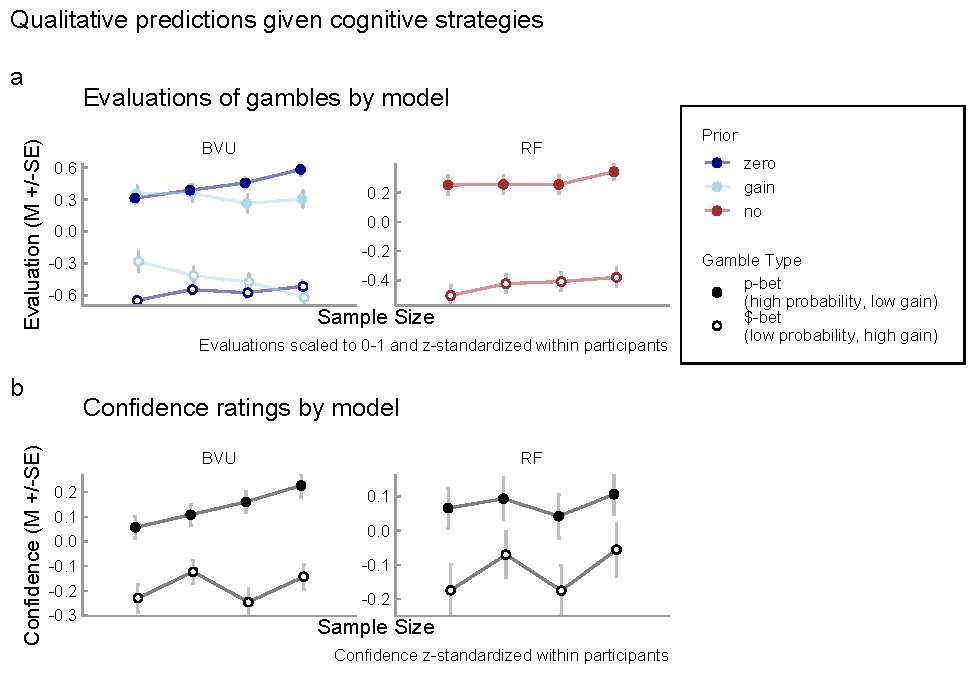
\includegraphics[width=.9\linewidth]{../figures/fig6-1} 

}

\caption{Mean evaluations by gamble type and best-fitting cognitive model and prior beliefs of the BVU model. \textit{BVU}$=$Bayesian value updating model, \textit{RF}$=$ Relative frequency model. Error bars indicate standard errors. Sample size categories see Table \ref{tab:Lotteries}. \textit{n} denotes the number of participants (of 80) that fall into the best-fitting model class. Evaluations are scaled to 0-1 and z-standardized at the individual level.}\label{fig:fig6}
\end{figure}

\textit{Predictions about confidence.}
\added[id=jj]{Regarding uncertainty about beliefs, the Bayesian model predicts that the uncertainty about beliefs reduces with more evidence. Thus in Bayesian lerners, confidence should increase with growing sample size. The relative frequency model makes no predictions about confidence. To test this, we classified participants into Bayesian and relative-frequency learners based on the best-fitting model. Mean confidence ratings of Bayesian-type learners, z-standardized within participants, did not increase from the extra small sample size ($M=-0.06, SD=1.00$), to the small sample size ($M=-0.00, SD=0.94$), medium sample size ($M=-0.01, SD=0.98$), and large sample size ($M=0.07, SD=1.01$, Figure \ref{fig:fig6}b), a linear regression model ($M_0$) without the cognitive model classification as predictor but with predictors sample size category and gambletype outperformed a regression including cognitive model category as predictor ($BF_{01}> 1000$).}


\end{document}
